\section{Parameter Values of the Preliminary KATRIN Energy Loss Model}
\label{sec:appendixKatrinElossElossModelParams}
The best-fit values, standard deviations and correlations of the fit parameters for the KATRIN model for the energy loss of electrons scattering off deuterium molecules as used in this thesis are listed below~\cite{Hannen2019_1}. The parameter names follow section~\ref{sec:katrinElossModel}.

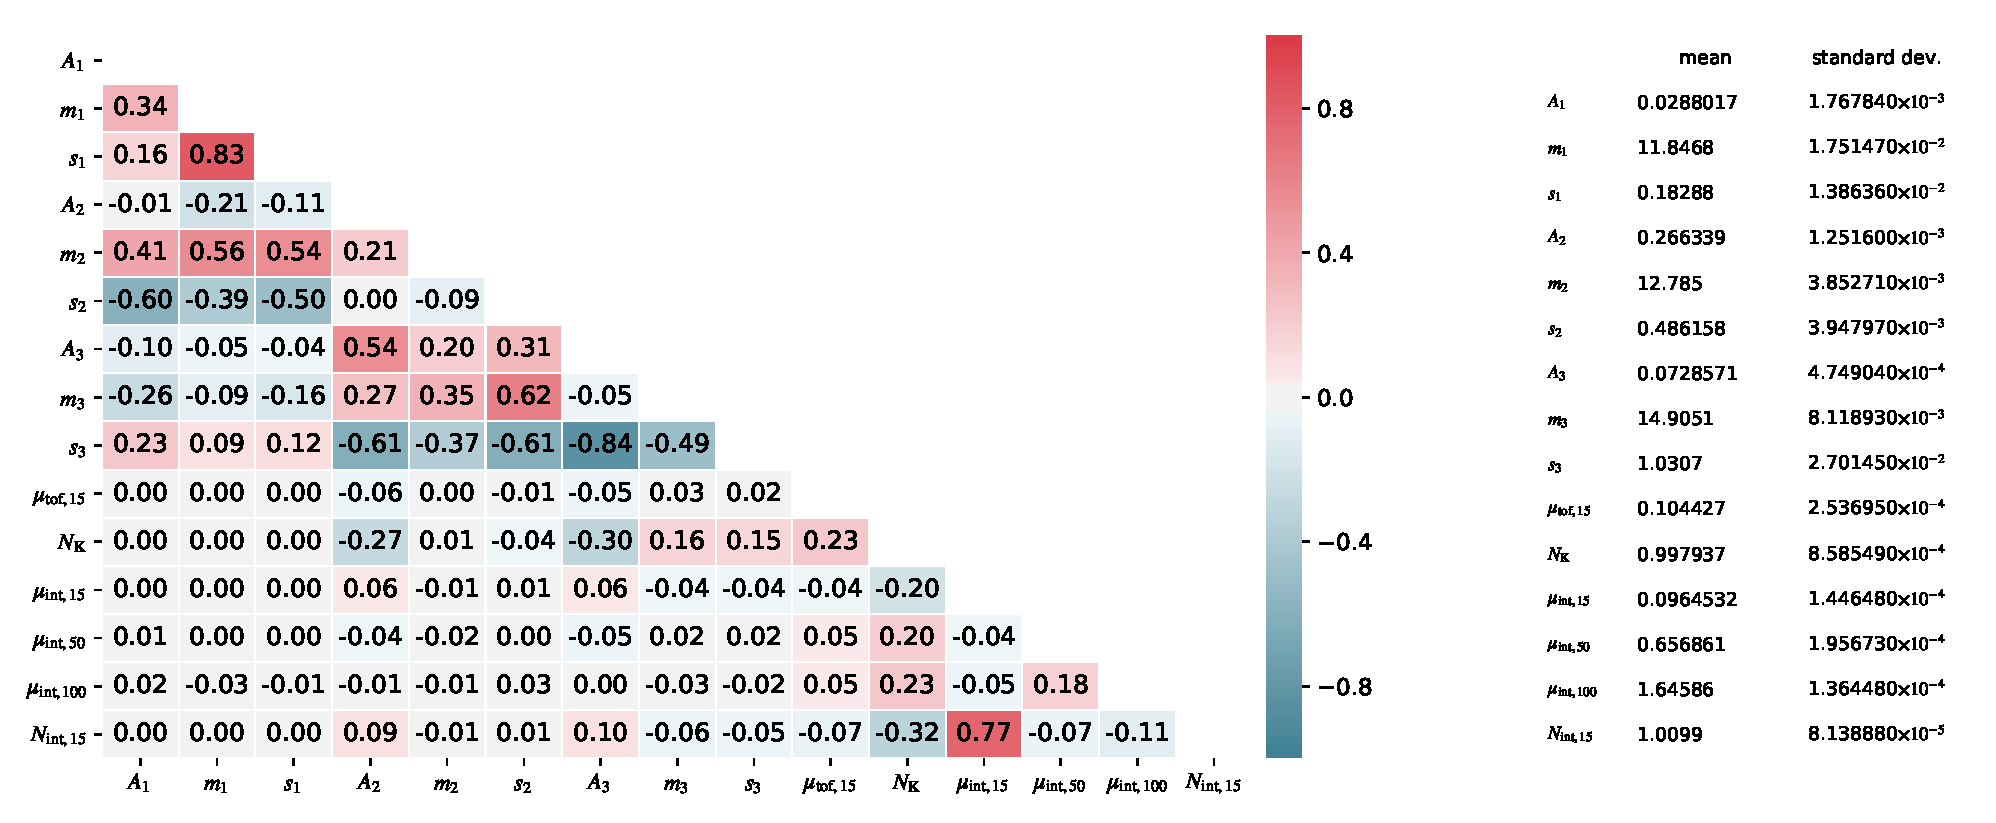
\includegraphics[width=\textwidth]{chapter/sensitivityStudyWithPreliminaryKatrinElossModel/appendix/fig/katrinElossParamValues.pdf}
\clearpage

\begin{samepage}
\section{Configuration of Sensitivity Study using the Preliminary KATRIN Energy Loss Model}
\label{sec:appendixKatrinElossSSCConfig}
The configuration of the \gls{ssc} module is listed below as used in the sensitivity study in chapter~\ref{sec:katrinEloss}.

\newcommand{\myModelConfigTableStrut}{\rule{0pt}{4ex}}
\begin{tabular}{ll}
	\toprule
	\textbf{\gls{wgts}} & \\
	\midrule
	gas column density & \SI{5e21}{molecules/m^2} (constant, no density profile) \\
	slices & 1 \\
	length & \SI{10.082}{m} \\
	tritium purity & \SI{95}{\percent} \\
	\myModelConfigTableStrut
	\textbf{Differential Spectrum} & \\
	\midrule
	final molecular states & by Saenz, emulating Doppler effect \\
	theo. corrections & screening, radiation (reference energy: molecular final states) \\
	Fermi function & approximately relativistic \\
	endpoint energy & \SI{18575}{eV} \\
	squared neutrino mass & \SI{0}{eV} \\
	\myModelConfigTableStrut
	\textbf{Energy Loss} & \\
	\midrule
	energy loss function & KATRIN or Aseev model \\
	inel. scattering cross section & \SI{3.456e-22}{m^2} \\
	elas. scattering & neglected \\
	\myModelConfigTableStrut
	\textbf{Transmission Function} & \\
	\midrule
	general configuration & relativistic, not detailed \\
	mag. field in analyzing plane & \SI{3e-4}{T} \\
	mag. field of pinch magnet & \SI{6}{T} \\
	mag. field in \gls{wgts} & \SI{3.6}{T} \\
	\myModelConfigTableStrut
	\textbf{Detector} & \\
	\midrule
	efficiency & \SI{95}{\percent} \\
	\myModelConfigTableStrut
	\textbf{MTD} & \\
	\midrule
	range & $[E_0-\SI{30}{eV},E_0+\SI{5}{eV}]$ \\
	duration & 3 years \\
	\bottomrule
\end{tabular}
\end{samepage}